\documentclass{standalone}

\usepackage{tikz}

\usetikzlibrary{
  calc
}

\begin{document}
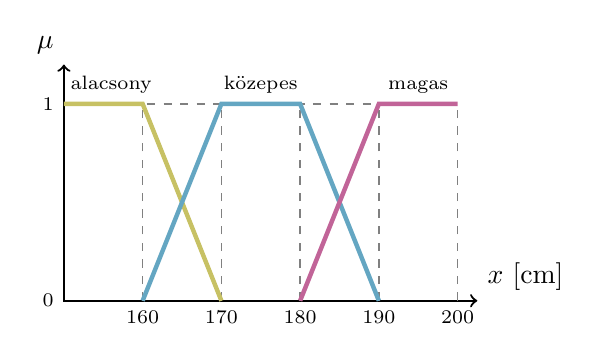
\begin{tikzpicture}[thick]
  \draw[to-to]
  (0,3) node[above left] {$\mu$}
  |- (5.25,0) node[above right] {$x$ [cm]};

  \draw[dashed, gray, semithick] (0,2.5) -- ++(5,0);
  \foreach \i in {1,2,3,4,5} {
      \draw[dashed, gray, semithick] (\i,0) -- ++(0,2.5);
    }
  \draw[ultra thick, yellow!50!gray] (0,2.5) -- ++(1,0) -- (2,0);
  \draw[ultra thick, cyan!50!gray] (1,0) -- ++(1,2.5) -- ++(1,0) -- (4,0);
  \draw[ultra thick, magenta!50!gray] (3,0) -- ++(1,2.5) -- ++(1,0);

  \begin{scope}[font=\scriptsize]
    \node[left] at (0,0) {0};
    \node[left] at (0,2.5) {1};
    \foreach \i/\h in {1/160,2/170,3/180,4/190,5/200} {
        \node[below] at (\i, 0) {\h};
      }

    \node[above] at (0.6,2.5) {alacsony};
    \node[above] at (2.5,2.5) {közepes};
    \node[above] at (4.5,2.5) {magas};
  \end{scope}
\end{tikzpicture}
\end{document}
